\documentclass{llncs}

\usepackage{booktabs}

\usepackage{graphicx}
\usepackage{caption}
\usepackage{subcaption}
\captionsetup{compatibility=false}

\usepackage{xcolor}
\usepackage{enumitem,amsmath,amssymb}
\usepackage{breakurl}    % used for \url and \burl
\usepackage[linesnumbered,vlined,ruled]{algorithm2e}
\def\defaultHypSeparation{\hskip.1in}

\usepackage{tikz}
%\usepackage{subfig}
\usepackage{array,booktabs,multirow}
\usepackage{placeins}

\usepackage{logictools}
\usepackage{prooftheory}
\usepackage{comment}
\usepackage{mathenvironments}
\usepackage{drawproof}

\DeclareMathOperator{\pebble}{P}
\DeclareMathOperator{\unpebble}{U}
\DeclareMathOperator{\pebbledAt}{pebbledAt}
\DeclareMathOperator{\peb}{peb}
\DeclareMathOperator{\free}{free}
\DeclareMathOperator{\ap}{ap}
\DeclareMathOperator{\relPerfomance}{relative\_performance}

\setlength{\belowbottomsep}{1ex}

\newcommand{\indexIn}[3]{\ensuremath{#1 \scriptstyle \in \{#2\ldots #3\} \displaystyle}}

\renewcommand{\arraystretch}{1.2}

\usetikzlibrary{patterns}

\renewcommand{\topfraction}{0.85}
\renewcommand{\textfraction}{0.1}
\renewcommand{\floatpagefraction}{0.75}

\newcommand{\defeq}{\mathrel{\mathop:}=}
\newcommand{\eqdef}{\mathrel{\mathop=}:}

\newcommand{\nodedistance}{0.55cm}
\newcommand{\nodedistanceThree}{0.6cm}
\newcommand{\nodedistanceTwo}{1.2cm}

\newcommand{\Vertices}[1]{V_{#1}}
\newcommand{\Edges}[1]{E_{#1}}
\newcommand{\Conclusion}[1]{\clause_{#1}}
\newcommand{\Premises}[2]{P_{#1}^{#2}}
\newcommand{\Children}[2]{C_{#1}^{#2}}
\newcommand{\Axioms}[1]{A_{#1}}

\newcommand{\axiom}[1]{\widehat{#1}}
\newcommand{\n}{v}
\newcommand{\raiz}[1]{\rho(#1)}

\newcommand{\pspace}[2]{s(#1,#2)}

\title{Greedy Pebbling: \\ 
Towards Proof Space Compression}

\author{
  Andreas Fellner 
  \thanks{Supported by the Google Summer of Code 2013 program.}
  \and 
  Bruno Woltzenlogel Paleo 
  \thanks{Supported by the Austrian Science Fund, project P24300.}
}

\authorrunning{A.\~Fellner \and B.\~Woltzenlogel Paleo}

\institute{
  \email{fellner.a@gmail.com} \ \ \ \email{bruno@logic.at} \\
  Theory and Logic Group \\
  Institute for Computer Languages \\
  Vienna University of Technology
}

\begin{document}

\maketitle

\setcounter{footnote}{0}

%%%%%%%%%%%%%%%%%%%%%%%%%%%%%%%%%%%%%%%%%
%%% Introduction %%%%%%%%%%%%%%%%%%%%%%%%
%%%%%%%%%%%%%%%%%%%%%%%%%%%%%%%%%%%%%%%%%
%\chapter{Introduction}
%\label{ch:introduction}
%%%%%%%%%%%%%%%%%%%%%%%%%%%%%%%%%%%%%%%%%

%\section{Introduction}

Proofs generated by SAT-solvers can be huge. 
Checking their correctness can not only take a long time but also consume a lot of memory. 
In an ongoing project for controller synthesis based on the extraction of interpolants from SMT-proofs \cite{Hofferek2013}, 
for example, post-processing a proof takes hours and may reach the limit of memory available today in a single node of a computer cluster (256GB). This issue is even more relevant in application scenarios in which the proof consumer, who is interested in independently checking the correctness of the proof, might have less available memory than the proof producer.
This is in part because, while the proof checker reads a usual proof file and checks the proof it contains, 
every proof node (containing a clause) that is loaded into memory has to be kept there until the end of the whole proof checking process, 
since the proof checker does not know whether a proof node will still need to be used and re-reading the proof file to reload and recheck proof nodes would be too time-consuming. 

To address this issue, recently proposed proof formats such as DRUP \cite{drup} and BDRUP \cite{bdrup} allow enriching a proof file with instructions that inform a proof checker when a proof node can be released from memory. Other proof formats, such as the TraceCheck format \cite{tracecheck} could also be enriched analogously. Such node deletion instructions can be added by a proof-generating SAT-solver during proof search in the periodic clean-up of its database of derived learned clauses; for every clause the SAT-solver deletes during this phase, this deletion can be recorded in the proof file. 

This paper explores the possibility of post-processing a proof in order to increase the amount of deletion instructions in the proof file. The more deletion instructions, the less memory the proof checker will need. Therefore, this \emph{deletion-during-proof-postprocessing} approach ought to be seen not as a replacement but rather as an independent complement to the \emph{deletion-during-proof-search} already performed by state-of-the-art proof-generating SAT-solvers.

The new methods proposed here exploit an analogy between proof checking and 
playing \emph{Pebbling Games} \cite{Kasai1979,Gilbert1980}. 
The particular version of pebbling game relevant for proof checking is defined precisely in Section \ref{sec:pebbling-game} and the analogy to proof checking is explained in detail in Section \ref{sec:pebblingchecking}. The proposed pebbling algorithms are greedy (Section \ref{sec:algorithms}) and based on heuristics (Section \ref{sec:heuristics}). As discussed in Sections \ref{sec:pebblingchecking} and \ref{sec:pebblingSAT}, approaches based on exhaustive enumeration or on encoding as a SAT problem would not fare well in practice.

The proof space compression algorithms described here are not restricted to proofs generated by SAT-solvers. They are general DAG pebbling algorithms, that could be applied to proofs represented in any calculus where proofs are directed acyclic graphs (including the special case of tree-like proofs). It is, nevertheless, in SAT and SMT that proofs tend to be largest and in most need of space compression. The underlying propositional resolution calculus (described in Section \ref{sec:Resolution}) satisfies the DAG requirement. The experiments (Section \ref{sec:experiments}) evaluate the proposed algorithms on thousands of SAT- and SMT-proofs.



%%%%%%%%%%%%%%%%%%%%%%%%%%%%%%%%%%%%%%%%%
%%% Resolution %%%%%%%%%%%%%%%%%%%%%%%%%%
%%%%%%%%%%%%%%%%%%%%%%%%%%%%%%%%%%%%%%%%%
%\chapter{Resolution}
%\label{ch:resolution}
%%%%%%%%%%%%%%%%%%%%%%%%%%%%%%%%%%%%%%%%%

%\section{Propositional Resolution Calculus}
\label{sec:resolution}

In this chapter, we will define the propositional resolution calculus.
Resolution is one of the most well known automated inference techniques and goes back to Robinson \cite{TODO}.
While it a pretty simple calculus with just one inference rule, proofs in that calculus tend to become big.
This property and its popularity make it a good target for applying proof compression to it.

Propositional resolution can be seen as a simplification of first-order logic resolution to propositional logic.
For basics about propositional logic, we refer the reader to \cite{TODO}.
For an extensive discussion of first-order logic resolution, we refer the reader to \cite{TODO}.

\begin{definition}[Literal and Clause]

A \emph{literal} is a propositional variable or the negation of a propositional variable. 
The \emph{complement} of a literal $\ell$ is denoted $\dual{\ell}$ (i.e. for any propositional variable $p$,
$\dual{p} = \neg p$ and $\dual{\neg p} = p$). 
The set of all literals is denoted by $\mathcal{L}$. 
A \emph{clause} is a set of literals. 
$\bot$ denotes the \emph{empty clause}.

\end{definition}

Clauses represent formulas by interpreting it as the conjunction of its literals.
Sets of clauses represent formulas by interpreting them as the disjunction of the interpreted clauses.
The propositional resolution calculus operates on propositional formulas in conjunctive normal form, which are formulas that are represented by a set of clauses.

\begin{definition}[Resolvent]

Let $C_1$ and $C_2$ be two clauses and $\ell$ be a literal, such that $\ell \in C_1$ and $\dual{\ell} \in C_2$.
The clause $C_1 \setminus \{\ell\} \cup C_2 \setminus \{\dual{\ell}\}$ is called the \emph{resolvent} of $C_1$ and $C_2$ w.r.t. $\ell$.

\end{definition}

In terms of proof calculi, axioms of the propositional resolution calculus are clauses and the single rule of the calculus is to derive a resolvent from previously derived clauses or axioms.
This work studies the syntactic and semantic structure of derivations in this calculus, which are formally defined in the following.

\begin{definition}[Resolution Derivation and Refutation]

Let $F = \{C_1, \ldots, C_n\}$ be a set of clauses.
The notion of a \emph{resolution derivation} for $F$ is defined inductively.
\begin{itemize}
	\item $\langle C_1, \ldots, C_n\rangle$ is a resolution derivation for $F$.
	\item If $\langle C_1, \ldots, C_m\rangle$ is a resolution derivation for $F$ then $\langle C_1, \ldots, C_{m+1} \rangle$ is a resolution derivation for $F$ if $C_{m+1}$ is a resolvent of $C_i$ and $C_j$ with $1 \leq i,j \leq m$.
\end{itemize}
A \emph{resolution refutation} is a resolution derivation containing the empty clause.

\end{definition}

The correctness of the resolution calculus can be formulated as the statement, that a propositional logic formula, represented as a set of clauses, is equivalent to all resolution derivations of it. 
Since the empty clause is unsatisfiable, a resolution derivation is unsatisfiable.
Therefore a resolution derivation of $F$ is a proof of the validity of $\neg F$.
We want to define resolution derivations in terms of graphs and call these objects proofs.

\begin{definition}[Proof] 
\label{def:proof}
A \emph{proof} $\varphi$ is a rooted labeled directed acyclic graph $\langle V,E,\n,\mathcal{L} \rangle$, such that
$\mathcal{L}$ maps nodes to clauses, $\n \in V$ is the root of the graph, 
such that $\langle V,E \rangle$ is a labeled directed acyclic graph whose edges are labeled with literals $\ell \in \mathcal{L}$, i.e. $E \subseteq V \times \mathcal{L} \times V$, $\n \in V$, $\clause$ is a clause 
and one of the following holds:

\begin{enumerate}
	\item $V = \{\n\}, E = \emptyset$
	\item \label{enum:resCase} There are proofs $\varphi_L = \langle V_L, E_L, \n_L,\clause_L \rangle$ and $\varphi_R = \langle V_R, E_R, \n_R, \clause_R \rangle$ such that there exists a literal
				$\ell$ such that $\dual{\ell} \in \Gamma_L$, $\ell \in \Gamma_R$, and let $\n \notin (V_L \cup V_R)$ then
		\begin{align*}
      V &= (V_L \cup V_R) \cup \{\n \} \\
      E &= E_L \cup E_R \cup
                    \left\{\n_L \xrightarrow{\dual{\ell}} \n , \n_R \xrightarrow{\ell} \n \right\} \\
     \Gamma &= \left( \clause_L \setminus \left\{ \dual{\ell} \right\} \right) \cup \left( \clause_R
                    \setminus \left\{ \ell \right\} \right)
    \end{align*}
		
\qed
\end{enumerate}
$\n$ is called the \emph{root} of $\varphi$ and $\clause$ its \emph{conclusion}.
$\varphi_L$ and $\varphi_R$ are \emph{premises} of $\varphi$ and $\varphi$ is a \emph{child} of $\varphi_L$ and $\varphi_R$.
$\Gamma$ is called the \emph{resolvent} of $\Gamma_L$ and $\Gamma_R$ with \emph{pivot} $\ell$.
A proof $\psi$ is a subproof of a proof $\varphi$, if there is a path from $\varphi$ to $\psi$ in the transitive closure of the premise relation.
A subproof $\psi$ of $\varphi$ which has no premises is an \emph{axiom} of $\varphi$.
$\Vertices{\varphi}$ and $\Axioms{\varphi}$ denote, respectively, the set of nodes and axioms of $\varphi$. $\Premises{\n}{\varphi}$ denotes the premises and $\Children{\n}{\varphi}$ the children of the subproof with root $\n$ in a proof $\varphi$. When a proof is represented graphically, the root is drawn at the bottom and the axioms at the top. The \emph{length} of a proof $\varphi$ is the number of nodes in $\Vertices{\varphi}$ and is denoted by $\plength{\varphi}$.
\end{definition}

\noindent
Note that in case \ref{enum:resCase} of Definition \ref{def:proof} $V_L$ and $V_R$ are not required to be disjunct. 
Therefore the underlying structure of a proof is a directed acyclic graph and not simply a tree. 
Modern SAT- and SMT-solvers, using techniques of conflict driven clause learning, produce proofs with a general DAG structure \cite{Bouton2009,Biere2009}.
The reuse of proof nodes plays a central role in proof compression \cite{Fontaine2011}.
Also note that a DAG corresponding to a proof has exactly one sink, which is called its root node, by definition.\\
For example a node of a proof $\langle V,E,\n,\clause \rangle$ will be meant to be some $s \in V$.
From hereon, if free from ambiguity, proofs and their underlying DAGs will not be distinguished. 


%%%%%%%%%%%%%%%%%%%%%%%%%%%%%%%%%%%%%%%%%
%%% Pebbling Game %%%%%%%%%%%%%%%%%%%%%%%
%%%%%%%%%%%%%%%%%%%%%%%%%%%%%%%%%%%%%%%%%
%\chapter{Pebbling Game}
%\label{ch:pebbling-game}
%%%%%%%%%%%%%%%%%%%%%%%%%%%%%%%%%%%%%%%%%

%\section{Pebbling Game}
\label{sec:pebbling-game}

%Todo: Discuss relation to resolution space complexity further
Pebbling games were introduced in the 1970's to model programming language expressiveness \cite{paterson1970comparative,Walker1973404} and compiler construction \cite{sethi1975complete}. 
More recently, pebbling games have been used to investigate various questions in parallel complexity \cite{chan2013pebble} and proof complexity \cite{ben2008short,Esteban200184,nordstrom2009narrow}. They are used to obtain bounds for space and time requirements and trade-offs between the two measures \cite{van1979move,ben2009size}. 
In this work we investigate space requirements when time is fixed.
Fixing time is a design choice, see Section \ref{sec:pebblingchecking}.
From hereon \textit{to pebble} means to mark a node with a pebble and \textit{to unpebble} means to remove the mark of a node.

\begin{definition}[Static Pebbling Game]
\label{def:pebbling-game}
The \emph{Static Pebbling Game} is played by one player on a DAG $G = (V,E)$ with one distinguished node $s \in V$.
The goal of the game is to pebble $s$, respecting the following rules:
\begin{enumerate}
	\item \label{rule:premises} A node $\n$ is pebbleable \emph{iff} all predecessors of $\n$ in $G$ are pebbled and $\n$ is currently not pebbled.
	\item \label{rule:unpebbling} Pebbled nodes can be unpebbled at any time.
	\item \label{rule:onlyonce} Once a node has been unpebbled, it can not be pebbled again later.
\end{enumerate}
%Only pebbled nodes can be unpebbled and only unpebbled nodes can be pebbled.
The game is played in rounds.
In each round the player makes a move by choosing a node $v \in V$, such that $v$ is pebbled or pebbleable.
The action of the player is to pebble $v$ if $v$ is pebbleable and to unpebble $v$ if it is pebbled.
Due to rule \ref{rule:premises} the action is uniquely defined.
\qed
\end{definition}

Note that as a consequence of rule \ref{rule:premises}, pebbles can be put on nodes without predecessors at any time.
Also note that rule \ref{rule:onlyonce} corresponds to fixing time requirements, as with this rule the number of rounds is $O(|V|)$.
Playing the game on a proof $\varphi$ means to play the game on the underlying DAG with the distinguished node being the root of $\varphi$.

\begin{definition}[Strategy]
\label{def:strategy}
A \emph{pebbling strategy} $\sigma$ for the Static Pebbling Game, played on a DAG $G = (V,E)$ and distinguished node $s$, is a sequence of moves $(\sigma_1,\ldots,\sigma_n)$ of the player such that $\sigma_n = s$.
\end{definition}

The following definition allows to measure how many pebbles are required to play the Static Pebbling Game on a given graph.

\begin{definition}[Pebbling number]
The \emph{pebbling number of a pebbling strategy} $(\sigma_1,\ldots,\sigma_n)$ is defined as 
$ max_{\indexIn{i}{1}{n}}|\{ \n \in V \mid \n \text{ is pebbled in round } i\}| $.
The \emph{pebbling number of a DAG $G$ and node $s$} is defined as the minimum pebbling number of all pebbling strategies for $G$ and $s$.
\end{definition}

Note that the definitions \ref{def:pebbling-game} and \ref{def:strategy} leave freedom when to do unpebbling moves.
With the aim of finding strategies with low pebbling numbers, there is a canonical way when to do these moves, as will be shown later.

\noindent
The \emph{Static Pebbling Game} from definition \ref{def:pebbling-game} differs from the Black Pebbling Game discussed in \cite{hertel2007black,pippenger1982advances} in two aspects. 
Firstly, the Black Pebbling Game does not include rule \ref{rule:onlyonce}. 
Excluding this rule allows for pebbling strategies with lower pebbling numbers (\cite{sethi1975complete} has an example on page 1), which can have the cost of exponentially more moves \cite{van1979move}.
Secondly, when pebbling a node in the Black Pebbling Game, one of its predecessors' pebbles can be used instead of a fresh pebble (i.e. a pebble can be moved). The trade-off when allowing to moving pebbles are discussed in \cite{van1979move}. Deciding whether the pebbling number of a graph $G$ and node $s$ is smaller than $k$ is PSPACE-complete in the absence of rule \ref{rule:onlyonce} \cite{gilbert1980pebbling} and NP-complete when rule \ref{rule:onlyonce} is included \cite{sethi1975complete}.



%%%%%%%%%%%%%%%%%%%%%%%%%%%%%%%%%%%%%%%%%
%%% Pebbling and Proof Checking %%%%%%%%%
%%%%%%%%%%%%%%%%%%%%%%%%%%%%%%%%%%%%%%%%%
%\chapter{Pebbling and Proof Processing}
%\label{ch:pebblingprocessing}
%%%%%%%%%%%%%%%%%%%%%%%%%%%%%%%%%%%%%%%%%

%\section{Pebbling and Proof Processing}
\label{sec:pebblingchecking}

The problem of processing a proof with minimal memory consumption is analogous to the problem of finding a pebbling strategy with minimal pebbling number.
Proof processing could be checking its correctness, manipulating it or extracting information from it.
The following definition makes the notion of proof processing formal.

\begin{definition}[Proof Processing]
\label{def:proof-processing}

Let $\varphi$ be a proof with nodes $V$ and $T$ be an arbitrary set.
We call a function $f: V \times T \times T \rightarrow T$ a \emph{processing function} if there is a function $g_f: V \rightarrow T$ such that for every $v \in V$ with $\Premises{v}{\varphi} = \emptyset$ (i.e. $v$ represents an axiom), $g_f(v) = f(v,t_1,t_2)$ for all $\{t_1,t_2\} \subseteq T$.
The \emph{apply function} $\ap: V \times T^{V\times T \times T} \rightarrow T$ is defined recursively as follows.
$$
\ap(\n,f) = \Big\{
\begin{array}{ll}
	f(\n,\ap(pr_1,f),\ap(pr_2,f)) &\text{ if } \n \text{ has premises } pr_1 \text{ and } pr_2\\
	g_f(\n) &\text{ otherwise}\\
\end{array}
$$

\emph{Processing a node} $\n$ with some processing function $f$ means computing the value $\ap(\n,f)$.
\emph{Processing a proof} means to process its root node.
\qed
\end{definition}

\begin{example}

Checking the correctness of a proof (i.e. checking for the absence of faulty resolution steps) can be checked in terms of the following processing function with $T = \{\top,\bot\}$ and $\wedge$ being the usual boolean and-operation.
$$
f(\n,w_1,w_2) = \left\{
\begin{array}{ll}
	\top & \text{ if $\n$ has no premises} \\
	w_1 \wedge w_2 &\text{ if the conclusion of $\n$ is a resolvent}\\
								 &\quad \text{ of the conclusions of its premises} \\
	\bot & \text{ otherwise}
\end{array}
\right.
$$
Processing a proof with this processing function yields $\top$ \emph{iff} the proof is a correct resolution proof.
\qed
\end{example}

In Section \ref{sec:pebbling-game} it was pointed out that strategies with minimal pebbling numbers may require to play exponentially many rounds.
Every round of the game corresponds to an I/O operation and, if the action of the player is to pebble a node, the processing of the node.
The goal of proof compression is to reduce the hardness of proof processing, therefore requiring exponentially many I/O operations and processing steps is not a viable option.
That is the reason why we chose the Bounded Pebbling Game for our purpose.
In the Bounded Pebbling Game the number of rounds is essentially the number of nodes.

In order to process a node, the results of processing its premises are used and therefore have to be stored in memory.
The requirement of having premises in memory corresponds to rule \ref{rule:premises} of the Bounded Pebbling Game. 
Processing a node and I/O operations are typically more expensive than extra memory consumption, therefore in our setting every node can be processed only once, which corresponds to rule \ref{rule:onlyonce}.
A node that has been processed can be removed from memory, which corresponds to rule \ref{rule:unpebbling}.
Note that removing a node and its results too early in combination with \ref{rule:onlyonce} makes it impossible to process the whole proof.
The best moment for removing a node from memory is canonical, as shown later in this chapter.

Definition \ref{def:proof-processing} leaves freedom in what order to process nodes.
The order in which nodes are processed is essential for the memory consumption, just like the order of pebbling nodes in the pebbling game is essential for the pebbling number.
The following definition allows us to relate pebbling strategies with orderings of nodes.

\begin{definition}[Topological Order]
\label{def:topological-order}
A topological order of a proof $\varphi$ is a total order relation $\prec$ on $\Vertices{\varphi}$, such that 
$\text{for all } \n \in \Vertices{\varphi} \text{, for all } p \in \Premises{\n}{\varphi}:
p \prec v$.
A pebbling strategy $\sigma = (\sigma_1,\ldots,\sigma_n)$ \emph{respects} a topological order $\prec$ if $j < i$ \emph{iff} $\sigma_j \prec \sigma_i$.
\qed
\end{definition}

A topological order $\prec$ of a proof $\varphi$ can be represented as a sequence $(v_1,\dots,v_n)$ of proof nodes, by defining $\prec \defeq \{(v_i,v_j) \mid 1 \leq i < j \leq n\}$. 
This sequence can be interpreted as a particular pebbling strategy for the game played on $\varphi$.
The requirement of topological orders to order premises higher than their children corresponds to rule \ref{rule:premises} of the Bounded Pebbling Game.
The antisymmetry together with the fact that $V = \{v_1,\dots,v_n\}$ corresponds to rule \ref{rule:onlyonce}.
The only thing missing are the unpebbling moves.
The following theorem states that unpebbling moves are given implicit, when the goal is to find strategies with small pebbling numbers.

%TODO: remove the ugly k
\begin{definition}[Canonical Topological Pebbling Strategy]
The \emph{canonical topological pebbling strategy} $\sigma$ for a proof $\varphi$, its root node $s$ and a topological order $\prec$ represented as a sequence $(v_1,\dots,v_n)$ is defined recursively:
$$
\begin{array}{l}
\sigma_1 = p(v_1) \\
\sigma_i = 
	\left\{
	\begin{array}{ll}
		u(v_j) & \text{ if there exists $j$ such that for all }v \in \Children{v_j}{\varphi}: \\
		       & \quad \text{ there exists }k < i, \sigma_k = p(v) \text{ and }\\
					 & \quad \text{ for all } l: k < l < i, \sigma_l \neq u(v_j) \\
		p(v_j) & \text{ otherwise where } j = min(k \mid \text{ for all }l < i: \sigma_l \neq p(v_k))
	\end{array}
	\right.
\end{array}
$$
\qed
\end{definition}

The following theorem shows that unpebbling moves can be omitted from strategies for the Bounded Pebbling Game, when the goal is to produce strategies with low pebbling numbers.

\begin{theorem}
\label{theorem:canonical}
The canonical pebbling strategy has the minimum pebbling number among all pebbling strategies that respect the topological order $\prec$.
\end{theorem}
\begin{proof} (Sketch)
All the pebbling strategies respecting $\prec$ differ only w.r.t. their unpebbling moves.
Consider the unpebbling of an arbitrary node $v$ in the canonical pebbling strategy. Unpebbling it later could only possibly increase the pebble number. To reduce the pebble number, $v$ would have to be unpebbled earlier than some preceding pebbling move. But, by definition of canonical pebbling strategy, the immediately preceding pebbling move pebbles the last child of $v$ w.r.t. $\prec$. Therefore, unpebbling $v$ earlier would make it impossible for its last child to be pebbled later without violating the rules of the game.
\qed
\end{proof}

As a consequence of Theorem \ref{theorem:canonical} is that finding pebbling strategies with low pebbling numbers can be reduced to constructing topological orders.
The memory required to process a proof using some topological order can be measured by the pebbling number of the pebbling strategy corresponding to the order.

\begin{definition}[Space]
\label{def:space measure}
The \emph{space} $\pspace{\varphi}{\prec}$ 
of a proof $\varphi$ and a topological order $\prec$ is the pebbling number of the canonical topological pebbling strategy of $\varphi$, its root and $\prec$.
\qed
\end{definition}

The problem of compressing the space of a proof $\varphi$ and a topological order $\prec$ is the problem of finding another topological order $\prec'$ such that $\pspace{\varphi}{\prec'} < \pspace{\varphi}{\prec}$. The following theorem shows that the number of possible topological orders is very large; hence, enumeration is not a feasible option when trying to find a good topological order.

\begin{theorem}
\label{theorem:enumeration}
There is a sequence of proofs $(\varphi_1,\ldots,\varphi_m,\ldots)$ such that $\plength{\varphi_m} \in O(m)$ and $|T(\varphi_m)| \in \Omega(m!)$, where $T(\varphi_m)$ is the set of possible topological orders for $\varphi_m$.
\end{theorem}
\begin{proof}
Let $\varphi_m$ be a perfect binary tree with $m$ axioms. Clearly, $\plength{\varphi_m} = 2m-1$.
Let $(\n_1,\ldots,\n_n)$ be a topological order for $\varphi_m$. 
Let $\Axioms{\varphi} = \{\n_{k_1},\ldots,\n_{k_m}\}$, then $(\n_{k_1},\ldots,\n_{k_m},\n_{l_1},\ldots,\n_{l_{n-m}})$, where $(l_1,\ldots,l_{n-m}) = (1,\ldots,n) \setminus (k_1,\ldots,k_m)$, is a topological order as well. 
Likewise, $(\n_{\pi({k_1})},\ldots,\n_{\pi({k_m})},\n_{l_1},\ldots,\n_{l_{n-m}})$ is a topological order, for every permutation $\pi$ of $\{k_1,\ldots,k_m\}$. There are $m!$ such permutations, so the overall number of topological orders is at least factorial in $m$ (and also in $n$).
\end{proof}



%%%%%%%%%%%%%%%%%%%%%%%%%%%%%%%%%%%%%%%%%
%%% Pebbling as a Satisfiability Problem 
%%%%%%%%%%%%%%%%%%%%%%%%%%%%%%%%%%%%%%%%%
%\chapter{Pebbling as a Satisfiability Problem}
%\label{ch:pebblingSAT}
%%%%%%%%%%%%%%%%%%%%%%%%%%%%%%%%%%%%%%%%%

%\section{Pebbling as a Satisfiability Problem}
\label{sec:pebblingSAT}

To find the pebble number of a proof, the question whether the proof can be pebbled using no more than $k$ pebbles can be encoded as a propositional satisfiability problem.
In this section let $\varphi$ be a proof with nodes $\n_1,\ldots,\n_n$ and let $\n_n$ be its root. 
Due to rule \ref{rule:onlyonce} of the Bounded Pebbling Game, the number of moves that pebble nodes is exactly $n$ and due to theorem \ref{theorem:canonical} determining the order of these moves is enough to define a strategy. 

In our SAT encoding, for every $x \in \{1,\ldots,k\}$, every $j \in \{1,\ldots,n\}$ and every $t \in \{0,\ldots,n\}$ there is a propositional variable $p_{x,j,t}$. 
The variable $p_{x,j,t}$ being mapped to $\top$ by a valuation is interpreted as the fact that in the $t$'th round of the game node $v_j$ is marked with pebble $x$.
Round $0$ is interpreted as the initial setting of the game before any move has been done.

For pebbling strategies, it is not relevant which of the $k$ pebbles is on a node.
Therefore one could also think of an encoding where true variables simply mean that a node is pebbled.
However, such an encoding would require exponentially many clauses (in $k$) when limiting the number of pebbles used in a round.

\begin{definition}[Pebbling SAT encoding]
%The following constraints, combined conjunctively, are satisfiable \textit{iff} there is a pebbling strategy $\sigma$ for $\varphi$ with pebbling number smaller or equal $k$. 
%In case the formula is satisfiable, a pebbling strategy can be read off from any satisfying assignment.
The conjunction of the following four constraints expresses the existence of a pebbling strategy for $\varphi$ with pebbling number smaller or equal $k$.

\begin{enumerate}
	\item The root is pebbled in the last round
				$$\Psi_1 = \bigvee_{x = 1}^k p_{x,n,n}$$
				
	\item No node is pebbled initially\\
				$$\Psi_2 = \bigwedge_{x = 1}^k \bigwedge_{j = 1}^n \left(\neg p_{x,j,0} \right)$$

	\item A pebble can only be on one node in one round
				$$\Psi_3 = \bigwedge_{x = 1}^k \bigwedge_{j = 1}^n \bigwedge_{t = 1}^n \left( p_{x,j,t} \rightarrow \bigwedge_{i = 1, i \neq j}^n \neg p_{x,i,t} \right)$$ 
				
	\item \label{c:pebble} For pebbling a node, its premises have to be pebbled the round before and only one node is being pebbled each round.\\
				\begin{align*}
					\Psi_4 = \bigwedge_{x = 1}^k \bigwedge_{j = 1}^n \bigwedge_{t = 1}^n & \Bigg( \left(\neg p_{x,j,t} \wedge p_{x,j,(t+1)} \right)\rightarrow \\
					&\bigg( \bigwedge_{i \in \Premises{j}{\varphi}} \bigvee_{y = 1, y \neq x}^k p_{y,i,t} \bigg) \wedge 
					\bigg( \bigwedge_{i = 1}^n \bigwedge_{y = 1, y \neq x}^k \neg \left( \neg p_{y,i,t} \wedge p_{y,i,(t+1)} \right) \bigg) \Bigg)
				\end{align*}
				
\end{enumerate}

The sets $\Axioms{\varphi}$ and $\Premises{j}{\varphi}$ are to be understood as sets of indices of the respective nodes.

\end{definition}

\noindent
This encoding is polynomial, both in $n$ and $k$. However constraint \ref{c:pebble} accounts to $O(n^3*k^2)$ clauses. 
Even small resolution proofs have more than $1000$ nodes and pebble numbers bigger than $100$, which adds up to $10^{13}$ clauses for constraint \ref{c:pebble} alone. 
Therefore, although theoretically possible to play the pebbling game via SAT-solving, this is practically infeasible for compressing proof space.
The following theorem proves the correctness of the encoding.

\begin{theorem}[Correctness of pebbling SAT encoding]

$\Psi = \Psi_1 \wedge \Psi_2 \wedge \Psi_3 \wedge \Psi_4$ is satisfiable if and only if there exists a pebbling strategy using no more than $k$ pebbles

\end{theorem}

\begin{proof}

\emph{Suppose $\Psi$ is satisfiable} and let $\mathcal{I}$ be a satisfying variable assignment in form of the set of true variables.
We will use $P(x,j,t)$ as an abbreviation for $p_{x,j,(t-1)} \notin \mathcal{I}$ and $p_{x,j,t} \in \mathcal{I}$.
Since $\mathcal{I}$ satisfies $\Psi_3$, in $P(x,j,t)$ $x$ is uniquely defined by $j$ and $t$ and we can write $P(j,t)$ instead.
We will prove the following assertion.
For every $t \in \{1,\ldots,n\}$ there exists exactly one $j \in \{1,\ldots,n\}$ such that $P(j,t)$.

%Every node, expect the root itself, is a recursive ancestor of the proof root.
$\Psi_1$ states that the root $v_n$ has to be pebbled in the last round and $\Psi_2$ states that no node is pebbled initially.
So for $n$ there has to be a $t \in \{1,\ldots,n\}$ such that $P(n,t)$.
$\mathcal{I}$ satisfies $\Psi_4$, therefore for every predecessor of $v_j$ of $v_n$ there exists $x \in \{1,\ldots,k\}$ such that $p_{x,j,(t-1)}$.
Using the same argument for $v_j$ as for $v_n$ there has to be a $t' \in \{1,\ldots,(t-1)\}$ such that $P(j,t')$.
Every node of the proof is a recursive ancestor of the root, therefore for every $j \in \{1,\ldots,n\}$ there exists at least one $t \in \{1,\ldots,n\}$ such that $P(n,t)$.
For every $t \in \{1,\ldots,n\}$, $\Psi_4$ ensures that if $P(n,t)$ then there is no $i \in \{1,\ldots,n\}, i \neq j$ such that $P(i,t)$, which proves the assertion.
The assertion implies the existence of a bijection $\tau : \{1,\ldots,n\} \rightarrow \{v_1,\ldots,v_n\}$ such that $\tau(n) = v_n$ and $\tau(t) = j$ \emph{iff} $P(j,t)$.
Therefore $\sigma := \{\tau(1),\ldots,\tau(n)\}$ is well defined.
$\sigma$ is a pebbling strategy, because $\tau(n) = v_n$, rule \ref{rule:premises} is obeyed because of $\Psi_4$, rule \ref{rule:unpebbling} is obeyed, because unpebbling moves are given implicitly (see Theorem \ref{theorem:canonical}) and rule \ref{rule:onlyonce} is obeyed because $\tau$ is a bijection.
$\Psi_3$ being satisfied ensures that $\sigma$ uses no more than $k$ pebbles.

\emph{Suppose there is a pebbling strategy $\sigma$ using no more than $k$ pebbles}. Let the function $\free: \{1,\ldots,n\} \rightarrow 2^{\{1,\ldots,k\}} \setminus \emptyset$ be defined recursively as follows and $\peb(t) = \min(\free(t)).$

$$
\free(t) = \left\{
  \begin{array}{ll}
    \{1,\ldots,k\} & : t = 1\\
    \free(t-1) \setminus \{\peb(t-1)\} \quad \cup & : otherwise\\
		\Big\{\peb(s) \mid \sigma_{s} \in \Premises{\sigma_{t-1}}{\varphi}, s \in \{1,\ldots,t-2\} \text{ and for all } v \in \Children{\sigma_{s}}{\varphi}&\\
		\text{ there exists } r \in \{1,\ldots,t-1\}: \sigma_{r} = v \Big\}&
  \end{array}
\right.
$$

Intuitively, $\free(.)$ keeps track of the unused pebbles in each round.
If a pebble is placed on a node, it is not free anymore.
Pebbles are made free again by unpebbling moves, which correspond to the second set in the recursive definition of $\free(.)$.
Since $\sigma$ uses no more than $k$ pebbles, $\free(.)$ is well defined.

Let $\mathcal{I}$ be a set of variables of $\Psi$ defined as follows.
$p_{x,j,t} \in \mathcal{I}$ \emph{iff} $t > 0$ and there exists $s \in \{1,\ldots,t\}$ such that $\peb(s) = x$, $\sigma_s = v_j$ and for all $r \in \{s+1,\ldots,t\}: x \notin \free(r)$.
$\mathcal{I}$ is a satisfying assignment for $\Psi$.
$\Psi_1$ is satisfied, because $\sigma_n = v_n$, therefore trivially $p_{\peb(n),n,n} \in \mathcal{I}$.
Clearly $\Psi_2$ is satisfied by $\mathcal{I}$ as no variables with $t = 0$ are included in $\mathcal{I}$.
To see that $\Psi_3$ is satisfied, suppose there exist $x,t,i,j$ such that $i \neq j$ and $\{p_{x,j,t},p_{x,i,t}\} \subseteq \mathcal{I}$.
Then by definition of $\mathcal{I}$ there exist unique $t_1$ and $t_2$ such that $\peb(t_1) = x, \sigma_{t_1} = v_j$ and $\peb(t_2) = x, \sigma_{t_2} = v_i$.
From $i \neq j$ follows $v_i \neq v_j$, therefore $t_1 \neq t_2$ w.l.o.g. suppose $t_1 > t_2$.
From $\peb(t_2) = x$, $p_{x,i,t} \in \mathcal{I}$ and $t \geq t_1 > t_2$ follows $x \notin \free(t_1)$, which is a contradiction to $\peb(t_1) = x$.
Let $P(x,j,t)$ be defined as above. Then from $P(x,j,t)$ follows $\peb(t) = x$ and $\sigma_t = v_j$.
Rule \ref{rule:premises} of the Bounded Pebbling Game ensures that there if $P(x,j,t)$ is true, then there exists a $y \{1,\ldots,k\} \setminus \{x\}$ such that $p_{y,i,t-1} \in \mathcal{I}$.
Suppose $P(x,j,t)$ and $P(y,i,t)$ both hold for some $t$, $x \neq y$ and $i \neq j$, then $y = \peb(t) = x$ and $v_j = \sigma_t = v_i$ are both contradictions. 
Therefore also $\Psi_4$ is satisfied by $\mathcal{I}$.

\end{proof}

%%%%%%%%%%%%%%%%%%%%%%%%%%%%%%%%%%%%%%%%%
%%% Greedy Pebbling Algorithms %%%%%%%%%%
%%%%%%%%%%%%%%%%%%%%%%%%%%%%%%%%%%%%%%%%%
%\chapter{Greedy Pebbling Algorithms}
%\label{ch:algorithms}
%%%%%%%%%%%%%%%%%%%%%%%%%%%%%%%%%%%%%%%%%

\section{Greedy Pebbling Algorithms}
\label{sec:algorithms}

Theorem \ref{theorem:enumeration} and the remarks in the end of section \ref{sec:PebblingAsSat} indicate that obtaining an optimal topological order either by enumerating topological orders or by encoding the problem as a satisfiability problem is impractical. 
This section presents two greedy algorithms that aim at finding good though not necessarily optimal topological order. 
They are both parameterized by some heuristic described in Section \ref{sec:heuristics}, but differ in the traversal direction in which the algorithms operate on proofs.

\subsection{Top-Down Pebbling}

\algo{Top-Down} Pebbling (Algorithm \ref{algo:TDpebbling}) constructs a topological order of a proof $\varphi$ by traversing it from its axioms to its root node.
This approach closely corresponds to how a human would play the pebbling game. 
A human would look at the nodes that are available for pebbling in the current round of the game, choose one of them to pebble and remove pebbles if possible.
Similarly the algorithm keeps track of pebblable nodes in a set $N$, initialized as $\Axioms{\varphi}$.
When a node $\n$ is pebbled, it is removed from $N$ and added to the sequence representing the topological order. The children of $\n$ that become pebbleable are added to $N$.
When $N$ becomes empty, all nodes have been pebbled once and a topological order has been found.


\begin{algorithm}[h]
  \KwIn{proof $\varphi$}
  \KwOut{sequence of nodes $S$ representing a topological order $\prec$ of $\varphi$}
	
	$S = ()$; \tcp*[f]{the empty sequence} \\
	$N = \Axioms{\varphi}$; \tcp*[f]{initialize pebbleable nodes with Axioms}
	
  \While{$N$ is not empty}{
    choose $\n \in N$ heuristically\;
		$S = S ::: (\n)$; \tcp*[f]{$:::$ is the concatenation of sequences}\\
		$N = N \setminus \{\n\}$\;
		\For(\tcp*[f]{check whether $c$ is now pebbleable}){\KwSty{each} $c \in \Children{\n}{\varphi}$}{ 
			\If{$\forall p \in \Premises{c}{\varphi}: p \in S$}
					{$N = N \cup \{c\}$\;}
					}
  }
	
	\Return $S$\;
	
  \caption[.]{\FuncSty{Top-Down Pebbling}}
  \label{algo:TDpebbling}
\end{algorithm}

\begin{example}
\label{example:topdown}

\begin{figure}[tb]
	\makebox[\textwidth][c]{
	\begin{minipage}{.33\textwidth}
		\begin{tikzpicture}[node distance=\nodedistance]
			\proofnodeBW{root};
			\proofnodeBW[above left of = root,xshift=-\nodedistance]{n7};
			\proofnodeBW[above right of = n7,xshift=\nodedistance]{n6};
			\proofnodeBW[above left of = n7]{n3};
			\proofnodeBW[above right of = root,xshift=\nodedistance]{n12};
			\proofnodeBW[above right of = n12]{n10};
			\withchildrenBW{n3}{n1}{n2};
			\withchildrenBW{n10}{n8}{n9};
			\proofnodeBW[above right of = n2]{n4};
			\proofnodeBW[above left of = n8]{n5};
			\drawchildren{n6}{n4}{n5};
			\withchildrenBW{n4}{e1}{e2};
			\withchildrenBW{n5}{e3}{e4};
			\drawchildren{root}{n7}{n12};
			\drawchildren{n7}{n3}{n6};
			\drawchildren{n12}{n6}{n10};
			\blacknode{n3};
			\node [yshift = 1.5mm] (cap1) at (n1.north) {\small{1}};
			\node [yshift = 1.5mm] (cap2) at (n2.north) {\small{2}};
			\node [yshift = 1.5mm] (cap3) at (n3.north) {\small{3}};
			\node [yshift = 1.5mm] (cap4) at (e1.north) {\small{4?}};
			\node [yshift = 1.5mm] (cap4) at (e2.north) {\small{4?}};
			\node [yshift = 1.5mm] (cap5) at (e3.north) {\small{4?}};
			\node [yshift = 1.5mm] (cap5) at (e4.north) {\small{4?}};
			\node [yshift = 1.5mm] (cap6) at (n8.north) {\small{4?}};
			\node [yshift = 1.5mm] (cap7) at (n9.north) {\small{4?}};
		\end{tikzpicture}
	\end{minipage}%
	\begin{minipage}{.33\textwidth}
		\begin{tikzpicture}[node distance=\nodedistance]
			\proofnodeBW{root};
			\proofnodeBW[above left of = root,xshift=-\nodedistance]{n7};
			\proofnodeBW[above right of = n7,xshift=\nodedistance]{n6};
			\proofnodeBW[above left of = n7]{n3};
			\proofnodeBW[above right of = root,xshift=\nodedistance]{n12};
			\proofnodeBW[above right of = n12]{n10};
			\withchildrenBW{n3}{n1}{n2};
			\withchildrenBW{n10}{n8}{n9};
			\proofnodeBW[above right of = n2]{n4};
			\proofnodeBW[above left of = n8]{n5};
			\drawchildren{n6}{n4}{n5};
			\withchildrenBW{n4}{e1}{e2};
			\withchildrenBW{n5}{e3}{e4};
			\drawchildren{root}{n7}{n12};
			\drawchildren{n7}{n3}{n6};
			\drawchildren{n12}{n6}{n10};
			\blacknode{n3};
			\blacknode{n8};
			\node [yshift = 2mm] (cap1) at (n1.north) {\small{1}};
			\node [yshift = 2mm] (cap2) at (n2.north) {\small{2}};
			\node [yshift = 2mm] (cap3) at (n3.north) {\small{3}};
			\node [yshift = 2mm] (cap8) at (n8.north) {\small{4}};
		\end{tikzpicture}
	\end{minipage}%
	\begin{minipage}{.33\textwidth}
	\begin{tikzpicture}[node distance=\nodedistance]
			\proofnodeBW{root};
			\proofnodeBW[above left of = root,xshift=-\nodedistance]{n7};
			\proofnodeBW[above right of = n7,xshift=\nodedistance]{n6};
			\proofnodeBW[above left of = n7]{n3};
			\proofnodeBW[above right of = root,xshift=\nodedistance]{n12};
			\proofnodeBW[above right of = n12]{n10};
			\withchildrenBW{n3}{n1}{n2};
			\withchildrenBW{n10}{n8}{n9};
			\proofnodeBW[above right of = n2]{n4};
			\proofnodeBW[above left of = n8]{n5};
			\drawchildren{n6}{n4}{n5};
			\withchildrenBW{n4}{e1}{e2};
			\withchildrenBW{n5}{e3}{e4};
			\drawchildren{root}{n7}{n12};
			\drawchildren{n7}{n3}{n6};
			\drawchildren{n12}{n6}{n10};
			\blacknode{n3};
			\blacknode{n10};
			\blacknode{n4};
			\blacknode{n5};
			\blacknode{e3};
			\blacknode{e4};
			\node [yshift = 2mm] (cap1) at (n1.north) {\small{1}};
			\node [yshift = 2mm] (cap2) at (n2.north) {\small{2}};
			\node [yshift = 2mm] (cap3) at (n3.north) {\small{3}};
			\node [yshift = 2mm] (cap4) at (n8.north) {\small{4}};
			\node [yshift = 2mm] (cap5) at (n9.north) {\small{5}};
			\node [yshift = 2mm] (cap6) at (n10.north) {\small{6}};
			\node [yshift = 2mm] (cap7) at (e1.north) {\small{7}};
			\node [yshift = 2mm] (cap8) at (e2.north) {\small{8}};
			\node [yshift = 2mm] (cap8) at (n4.north) {\small{9}};
			\node [yshift = 2mm] (cap7) at (e3.north) {\small{10}};
			\node [yshift = 2mm] (cap8) at (e4.north) {\small{11}};
			\node [yshift = 2mm] (cap8) at (n5.north) {\small{12}};
		\end{tikzpicture}
	\end{minipage}%
	}
	\caption{Top-Down Pebbling}
	\label{fig:TDP}
\end{figure}

Top-Down Pebbling often ends up finding a sub-optimal pebbling strategy regardless of the heuristic used. Consider the graph shown in Figure \ref{fig:TDP} and suppose that top-down pebbling has already pebbled the initial sequence of nodes $(1,2,3)$. 
For a greedy heuristic that only has information about pebbled nodes, their premises and children, all nodes marked with $4?$ are considered equally worthy to pebble next.
Suppose the node marked with $4$ in the middle graph is chosen to be pebbled next.
Subsequently, pebbling $5$ opens up the possibility to remove a pebble after the next move, which is to pebble $6$.
After that only the middle subgraph has to be pebbled. No matter in which order this is done, the strategy will use six pebbles at some point. 
One example sequence and the point where six pebbles are used are shown in the rightmost picture in Figure \ref{fig:TDP}.

\label{example:TDPIssue}
\end{example}

\subsection{Bottom-Up Pebbling}

\algo{Bottom-Up} Pebbling (Algorithms \ref{algo:BUpebbling} and \ref{algo:visit}) constructs a topological order of a proof $\varphi$ while traversing it from its root node to its axioms. The algorithm constructs the order by visiting nodes and their premises recursively. At every node $\n$ the order in which the premises of $\n$ are visited is decided heuristically. After visiting the premises, $n$ is added to the current sequence of nodes.
Since axioms do not have any premises, there is no recursive call for axioms and these nodes are simply added to the sequence. The recursion is started by a call to visit the root.
Since all proof nodes are ancestors of the root, the recursive calls will eventually visit all nodes once and a topological total order will be found.
Bottom-Up Pebbling corresponds to how the apply function $\ap(.)$ was defined in Section \ref{sec:pebblingchecking} with the addition of a visit order of the premises for each node and the omission of calls to previously processed nodes.

\SetKwFunction{KwVisit}{visit}

\begin{algorithm}[h]
  \KwIn{proof $\varphi$ with root node $r$}
  \KwOut{sequence of nodes $S$ representing a topological order $\prec$ of $\varphi$}
  \BlankLine

	$S = ()$\; \tcp*[f]{the empty sequence}\\
	$V = \emptyset$\;
	\Return \KwVisit{$\varphi$,$r$,$V$,$S$}\;

  \caption[.]{\FuncSty{Bottom-Up Pebbling}}
  \label{algo:BUpebbling}
\end{algorithm}

\begin{algorithm}[h]
  \KwIn{proof $\varphi$}
	\KwIn{node $\n$}
	\KwIn{set of visited nodes $V$} 
	\KwIn{initial sequence of nodes $S$}
  \KwOut{sequence of nodes}
	
	$V_1 = V \cup \{\n\}$;
	$N = \Premises{\n}{\varphi} \setminus V$; \tcp*[f]{Only unprocessed premises are visited} \\
	$S_1 = S$\;
	
  \While{$N$ is not empty}{
    choose $p \in N$ heuristically;
		$N = N \setminus p$\;
		$S_1 = S_1 ::: visit(\varphi,p,V,S)$; \tcp*[f]{$:::$ is the concatenation of sequences}
  }
	
	\Return $S_1 ::: (\n)$\;
	
  \caption[.]{\FuncSty{visit}}
  \label{algo:visit}
\end{algorithm}

%\newcommand{\nodedistance2}{0.6cm}
\begin{example}
Figure \ref{fig:BUP} shows part of an execution of \algo{Bottom-Up} Pebbling on the same proof as presented in Figure \ref{fig:TDP}.
Nodes chosen by the heuristic, to be processed before the respective other premise, are marked dashed. 
Suppose that similarly to the Top-Down Pebbling scenario, nodes have been chosen in such a way that the initial pebbling sequence is $(1,2,3)$.
However, the choice of where to go next is predefined by the dashed nodes. 
Consider the dashed child of node $3$. 
Since $3$ has been completely processed, the other premise of its dashed child is visited next. 
The result is that node the middle subgraph is pebbled while only one external node is pebbled, while it have been two in the Top-Down scenario. 
At no point more than five pebbles will be used for pebbling the root node, which is shown in the bottom right picture of the figure. This is independently of the heuristic choices.

Not that this example underlines the point of two observations: pebbling choices should be made local and hard subgraphs should be pebbled early.

\begin{figure}[tb]
	\makebox[\textwidth][c]{
		\begin{minipage}{0.4\textwidth}
			\begin{tikzpicture}[node distance=\nodedistanceThree]
				\proofnodeBW{root};
				\proofnodeBW[above left of = root,xshift=-\nodedistanceThree]{n7};
				\proofnodeBW[above right of = n7,xshift=\nodedistanceThree]{n6};
				\proofnodeBW[above left of = n7]{n3};
				\proofnodeBW[above right of = root,xshift=\nodedistanceThree]{n12};
				\proofnodeBW[above right of = n12]{n10};
				\withchildrenBW{n3}{n1}{n2};
				\withchildrenBW{n10}{n8}{n9};
				\proofnodeBW[above right of = n2]{n4};
				\proofnodeBW[above left of = n8]{n5};
				\drawchildren{n6}{n4}{n5};
				\withchildrenBW{n4}{e1}{e2};
				\withchildrenBW{n5}{e3}{e4};
				\drawchildren{root}{n7}{n12};
				\drawchildren{n7}{n3}{n6};
				\drawchildren{n12}{n6}{n10};
				\waitingnode{n7};
				\waitingnode{root};
				\blacknode{n3};
				\node [yshift = 2mm] (cap1) at (n1.north) {\small{1}};
				\node [yshift = 2mm] (cap2) at (n2.north) {\small{2}};
				\node [yshift = 2mm] (cap3) at (n3.north) {\small{3}};
			\end{tikzpicture}
		\end{minipage}%
		\begin{minipage}{0.4\textwidth}
			\begin{tikzpicture}[node distance=\nodedistance]
				\proofnodeBW{root};
				\proofnodeBW[above left of = root,xshift=-\nodedistanceThree]{n7};
				\proofnodeBW[above right of = n7,xshift=\nodedistanceThree]{n6};
				\proofnodeBW[above left of = n7]{n3};
				\proofnodeBW[above right of = root,xshift=\nodedistanceThree]{n12};
				\proofnodeBW[above right of = n12]{n10};
				\withchildrenBW{n3}{n1}{n2};
				\withchildrenBW{n10}{n8}{n9};
				\proofnodeBW[above right of = n2]{n4};
				\proofnodeBW[above left of = n8]{n5};
				\drawchildren{n6}{n4}{n5};
				\withchildrenBW{n4}{e1}{e2};
				\withchildrenBW{n5}{e3}{e4};
				\drawchildren{root}{n7}{n12};
				\drawchildren{n7}{n3}{n6};
				\drawchildren{n12}{n6}{n10};
				\waitingnode{n7};
				\blacknode{n3};
				\waitingnode{n6};
				\waitingnode{root};
				\node [yshift = 2mm] (cap1) at (n1.north) {\small{1}};
				\node [yshift = 2mm] (cap2) at (n2.north) {\small{2}};
				\node [yshift = 2mm] (cap3) at (n3.north) {\small{3}};
			\end{tikzpicture}
		\end{minipage}%
		}
		\makebox[\textwidth][c]{
		\begin{minipage}{0.4\textwidth}
			\begin{tikzpicture}[node distance=\nodedistanceThree]
				\proofnodeBW{root};
				\proofnodeBW[above left of = root,xshift=-\nodedistanceThree]{n7};
				\proofnodeBW[above right of = n7,xshift=\nodedistanceThree]{n6};
				\proofnodeBW[above left of = n7]{n3};
				\proofnodeBW[above right of = root,xshift=\nodedistanceThree]{n12};
				\proofnodeBW[above right of = n12]{n10};
				\withchildrenBW{n3}{n1}{n2};
				\withchildrenBW{n10}{n8}{n9};
				\proofnodeBW[above right of = n2]{n4};
				\proofnodeBW[above left of = n8]{n5};
				\drawchildren{n6}{n4}{n5};
				\withchildrenBW{n4}{e1}{e2};
				\withchildrenBW{n5}{e3}{e4};
				\drawchildren{root}{n7}{n12};
				\drawchildren{n7}{n3}{n6};
				\drawchildren{n12}{n6}{n10};
				\blacknode{n7};
				\blacknode{n6};
				\waitingnode{root};
				\node [yshift = 2mm] (cap1) at (n1.north) {\small{1}};
				\node [yshift = 2mm] (cap2) at (n2.north) {\small{2}};
				\node [yshift = 2mm] (cap3) at (n3.north) {\small{3}};
				\node [yshift = 2mm] (cap4) at (e1.north) {\small{5}};
				\node [yshift = 2mm] (cap5) at (e2.north) {\small{4}};
				\node [yshift = 2mm] (cap6) at (n4.north) {\small{6}};
				\node [yshift = 2mm] (cap7) at (e3.north) {\small{7}};
				\node [yshift = 2mm] (cap7) at (e4.north) {\small{8}};
				\node [yshift = 2mm] (cap7) at (n5.north) {\small{9}};
				\node [yshift = 2mm] (cap7) at (n6.north) {\small{10}};
			\end{tikzpicture}
		\end{minipage}%
		\begin{minipage}{0.4\textwidth}
			\begin{tikzpicture}[node distance=\nodedistanceThree]
				\proofnodeBW{root};
				\proofnodeBW[above left of = root,xshift=-\nodedistanceThree]{n7};
				\proofnodeBW[above right of = n7,xshift=\nodedistanceThree]{n6};
				\proofnodeBW[above left of = n7]{n3};
				\proofnodeBW[above right of = root,xshift=\nodedistanceThree]{n12};
				\proofnodeBW[above right of = n12]{n10};
				\withchildrenBW{n3}{n1}{n2};
				\withchildrenBW{n10}{n8}{n9};
				\proofnodeBW[above right of = n2]{n4};
				\proofnodeBW[above left of = n8]{n5};
				\drawchildren{n6}{n4}{n5};
				\withchildrenBW{n4}{e1}{e2};
				\withchildrenBW{n5}{e3}{e4};
				\drawchildren{root}{n7}{n12};
				\drawchildren{n7}{n3}{n6};
				\drawchildren{n12}{n6}{n10};
				\blacknode{n7};
				\blacknode{n6};
				\blacknode{n8};
				\blacknode{n9};
				\blacknode{n10};
				\waitingnode{root};
				\waitingnode{n12};
				\node [yshift = 2mm] (cap1) at (n1.north) {\small{1}};
				\node [yshift = 2mm] (cap2) at (n2.north) {\small{2}};
				\node [yshift = 2mm] (cap3) at (n3.north) {\small{3}};
				\node [yshift = 2mm] (cap4) at (e1.north) {\small{5}};
				\node [yshift = 2mm] (cap5) at (e2.north) {\small{4}};
				\node [yshift = 2mm] (cap6) at (n4.north) {\small{6}};
				\node [yshift = 2mm] (cap7) at (e3.north) {\small{7}};
				\node [yshift = 2mm] (cap7) at (e4.north) {\small{8}};
				\node [yshift = 2mm] (cap7) at (n5.north) {\small{9}};
				\node [yshift = 2mm] (cap7) at (n6.north) {\small{10}};
				\node [yshift = 2mm] (cap7) at (n8.north) {\small{11}};
				\node [yshift = 2mm] (cap7) at (n9.north) {\small{12}};
				\node [yshift = 2mm] (cap7) at (n10.north) {\small{13}};
			\end{tikzpicture}
		\end{minipage}%
			}
		\caption{Bottom-Up Pebbling}
		\label{fig:BUP}
\end{figure}
\label{example:BUP}
\end{example}



\subsection{Remarks about Top-Down and Bottom-Up Pebbling} %or: Which way to go?
\label{sec:TDvsBU}

In principle every topological order of a given proof can be constructed using Top-down or Bottom-up Pebbling. Both algorithms traverse the proof only once and have linear run-time in the proof length (assuming that the heuristic choice requires constant time). Example \ref{example:TDPIssue} shows a situation where \algo{Top-Down} Pebbling may pebble a node that is far away from the previously pebbled nodes. This results in a sub-optimal pebbling strategy.
As discussed in Example \ref{example:BUP}, \algo{Bottom-Up} Pebbling is more immune to this non-locality issue, because queuing up the processing of premises enforces local pebbling. This suggests that \algo{Bottom-Up} is better than \algo{Top-Down}, which is confirmed by the experiments in Section \ref{sec:exp}.



%%%%%%%%%%%%%%%%%%%%%%%%%%%%%%%%%%%%%%%%%
%%% Heuristics %%%%%%%%%%%%%%%%%%%%%%%%%%
%%%%%%%%%%%%%%%%%%%%%%%%%%%%%%%%%%%%%%%%%
%\chapter{Heuristics}
%\label{ch:heuristics}
%%%%%%%%%%%%%%%%%%%%%%%%%%%%%%%%%%%%%%%%%

%\section{Heuristics}
\label{sec:heuristics}

Heuristics are used in both pebbling algorithms to choose one node out of a set $N$. 
For Top-Down Pebbling, $N$ is the set of pebbleable nodes, and for Bottom-Up Pebbling, $N$ is the set of unprocessed premises of a node. 

\begin{definition}[Heuristic and Full Heuristics]

Let $\varphi$ be a proof with nodes $V$.
A \emph{heuristic} $h$ for $\varphi$ is a totally ordered set $S_h$ together with a \emph{node evaluation} function $e_h: V \rightarrow S_h$.
A \emph{full heuristic} for $\varphi$ is finite a sequence $(e_{h_1}, \ldots, e_{h_n})$ of heuristics such that the node evaluation $e_{h_n}$ is injective.
The \emph{choice} of the full heuristic for a set $N \subseteq V$ is some $\n \in N$ such that $\n = \mathit{argmax}_{\n \in N} e_{h_1}(\n)$ if $\n$ is unique and the choice of the full heuristic $(e_{h_2},\ldots,e_{h_n})$ for $\{\n \in N \mid \n = \mathit{argmax}_{\n \in N} e_{h_1}(\n)\}$. 
This process will eventually terminate, because of the limitation to $e_{h_n}$.

\end{definition}

Note that to satisfy the requirement for $e_{h_n}$, some trivial node evaluation like mapping nodes to their address in memory can be used.
In the next chapters we present heuristics, which are cheap to compute and are justified by relating them to the semantics of the Bounded Pebbling Game.
We will not elaborate on effects of reordering the heuristics within full heuristics.

\subsection{Number of Children Heuristic (``$Ch$'')}
\label{sec:children}
The \emph{Number of Children} heuristic uses the number of children of a node $\n$ as evaluation function, i.e. $e_h(\n) = |\Children{\n}{\varphi}|$ and $S_h = \mathbb{N}$.
The intuitive motivation for this heuristic is that nodes with many children will require many pebbles, and subproofs containing nodes with many children will tend to be more spacious.
Example \ref{example:hardfirst} shows the idea behind pebbling spacious subproofs early.

\subsection{Last Child Heuristic (``$Lc$'')}
\label{sec:lastchild}

As discussed in Section \ref{sec:pebbling-game} in the proof of Theorem \ref{theorem:canonical}, the best moment to unpebble a node $\n$ is as soon as its last child w.r.t. a topological order $\prec$ is pebbled. 
This insight is used for the \emph{Last Child} heuristic that chooses nodes that are last children of other nodes. 
Pebbling a node that allows another one to be unpebbled is always a good move. 
The current number of used pebbles (after pebbling the node and unpebbling one of its premises) does not increase.
It might even decrease, if more than one premise can be unpebbled.
For determining the number of premises of which a node is the last child, the proof has to be traversed once, using some topological order $\prec$.
Before the traversal, $e_h(\n) = 0$ for every node $\n$. 
During the traversal $e_h(\n)$ is incremented by 1, if $\n$ is the last child of the currently processed node w.r.t. $\prec$. 
For this heuristic $S_h = \mathbb{N}$.
To some extent, this heuristic is paradoxical: $\n$ may be the last child of a node $\n'$ according to $\prec$, but pebbling it early may result in another topological order $\prec^*$ according to which $\n$ is not the last child of $\n'$.
Nevertheless, sometimes the proof structure ensures that some nodes are the last child of another node irrespective of the topological order. An example is shown in Figure \ref{fig:forcedLC}, where the dashed line denotes a recursive predecessor relationship and the bottommost node is the last child of the top right node in every topological order.

\begin{figure}[h]
	\centering{
	\begin{tikzpicture}[node distance=1cm]
		\proofnodeBW{n4};
		\proofnodeBW[above left of = n4]{n3};
		
		%\proofnodeBW[above left of = n3]{n1};
		
		\proofnodeBW[above right of = n3]{n2};
		%\withchildrenBW{n3}{n1}{n2};
		%\drawchildren{n4}{n3}{n2};
		%\node[above left of=n3] (emptynode) {};
		%\draw[->,thick,cap=round,dashed] (n3) to (emptynode);
		\draw[->,thick,cap=round,dashed] (n3) to (n2);
		\draw[->,thick,cap=round] (n4) to (n2);
		\draw[->,thick,cap=round,dashed] (n4) to (n3);
		
	\end{tikzpicture}
	}
	\caption{Bottommost node as necessary last child of right topmost node}
	\label{fig:forcedLC}
\end{figure}


\subsection{Node Distance Heuristic (``$Dist(r)$'')}
\label{sec:distance}

In Example \ref{example:topdown} and Section \ref{sec:TDvsBU} it has been noted that Top-Down Pebbling may perform badly if nodes that are far apart are selected by the heuristic.
The \emph{Node Distance} heuristic prefers to pebble nodes that are close to pebbled nodes. It does this by calculating spheres with a radius up to the parameter $r$ around nodes.
A sphere $K_r^{G}(\n)$ with radius $r$ around the node $\n$ in the graph $G = (V,E)$ is the set $\{p \in V \mid v \text{ can be reached from } p \text{ visiting at most } r \text{ edges}\}$, where edges are considered undirected. 
The heuristic uses the following functions based on the spheres:
\begin{align*}
	d(\n) &\defeq \Bigg\{
	\begin{array}{l}
		-min(D) \text{ such that } D = \{r \mid K_r^{G}(\n)\text{ contains a pebbled node}\} \neq \emptyset\\
		\infty \text{ otherwise}
		\end{array}\\
	s(\n) &\defeq |K_{-d(\n)}^G(\n)|\\
	l(\n) &\defeq max_{\prec}K_{-d(\n)}^G(\n)\\
	e_h(\n) &\defeq (d(\n),s(\n),l(\n))
\end{align*}
where $\prec$ denotes the order of previously pebbled nodes.
So $S_h = \mathbb{Z} \times \mathbb{N} \times P$ together with the lexicographic order using, respectively, the natural smaller relation $<$ on $\mathbb{Z}$ and $\mathbb{N}$ and $\prec$ on $N$. The spheres $K_r(\n)$ can grow exponentially in $r$. Therefore the maximum radius has to be kept small.

\subsection{Decay Heuristics (``$Dc(h_u,\gamma,d,com)$'') }
\label{sec:decay}
Decay heuristics denote a family of meta heuristics. 
The idea is to not only use the evaluation of a single node, but also to include the evaluations of its premises.
Such a heuristic has four parameters: an underlying heuristic $h_u$ defined by an evaluation function $e_u$ together with a well ordered set $S_u$, a decay factor $\gamma \in \mathbb{R}^+ \cup \{0\}$, a recursion depth $d \in \mathbb{N}$ and a combining function $com: S_u^n \rightarrow S_u$ for $n \in \mathbb{N}$.
The resulting heuristic node evaluation function $e_h$ is defined with the help of the recursive function $rec$:
\begin{align*}
	rec(\n,0) &\defeq e_u(\n) \\
	rec(\n,k) &\defeq e_u(\n) + com(rec(p_1,k-1),\ldots,rec(p_n,k-1)) * \gamma\\
	& \text{ where } \Premises{\n}{\varphi} = \{p_1,\ldots,p_n\}\\
	% & \text{ and } k \in \{1,\ldots,d\} \\
	%rec(\n,k) &\defeq com(h_u(\n), rec(p_1,k-1)*\gamma,\ldots,rec(p_{n-1},k-1) * \gamma)\\ %might be better - I will try this in the experiments
	e_h(\n) &\defeq rec(\n,d) &
\end{align*}



%%%%%%%%%%%%%%%%%%%%%%%%%%%%%%%%%%%%%%%%%
%%% Experiments %%%%%%%%%%%%%%%%%%%%%%%%%
%%%%%%%%%%%%%%%%%%%%%%%%%%%%%%%%%%%%%%%%%
%\chapter{Experiments}
%\label{ch:experiments}
%%%%%%%%%%%%%%%%%%%%%%%%%%%%%%%%%%%%%%%%%

%\section{Experiments} 
\label{sec:experiments}

The experiments on the space compression algorithm were performed on four disjoint sets of proof benchmarks (Table \ref{tab:benchmarks}). 
TraceCheck$_1$ and TraceCheck$_2$ contain proofs produced by the SAT-solver PicoSAT \cite{Biere2008} on unsatisfiable benchmarks from the SATLIB. 
The proofs\footnote{SAT proofs: \url{www.logic.at/people/bruno/Experiments/2014/Pebbling/tc-proofs.zip}} are in the TraceCheck proof format, which is one of the three formats accepted at the \emph{Certified Unsat} track of the SAT-Competition.
veriT$_1$ and veriT$_2$ contain proofs produced by the SMT-solver VeriT \cite{Bouton2009} on unsatisfiable problems from the SMT-LIB. 
These proofs\footnote{SMT proofs: \scriptsize{\url{www.logic.at/people/bruno/Experiments/2014/Pebbling/smt-proofs.zip}}} are in a proof format that resembles SMT-LIB's problem format and they were translated into pure resolution proofs by considering every non-resolution inference as an axiom.

%%%%%%%%%%%%%%%%%%%%%%%%%%%%%%%%%%%%%%%%%%%%%%%%%%%%%%%%%%%%%%
%%%%%%%%%%%%%%% Benchmarks table &&&&&&&&&&&&&&&&&&&&&&&&&&&&&
%%%%%%%%%%%%%%%%%%%%%%%%%%%%%%%%%%%%%%%%%%%%%%%%%%%%%%%%%%%%%%

\begin{table}[tb]
	\centering
	\setlength{\tabcolsep}{8pt}
	\begin{tabular}{lrrr}
		\toprule
		%\textbf{Name} & \textbf{Number of proofs} & \textbf{Maximum length} & \textbf{Average length} \\ 
		\textbf{Name} & \textbf{Number of} & \textbf{Maximum} & \textbf{Average} \\ 
		              & \textbf{proofs}    & \textbf{length}  & \textbf{length} \\
		\midrule
		TraceCheck$_1$ & 2239 & 90756   & 5423   \\
		TraceCheck$_2$ & 215	& 1768249 & 268863 \\
    veriT$_1$ & 4187 & 2241042 & 103162 \\
    veriT$_2$ & 914  & 120075  & 5391  \\ 
		\bottomrule   
	\end{tabular}
	\caption{Proof benchmark sets}
	\label{tab:benchmarks}
\end{table}

%%%%%%%%%%%%%%%%%%%%%%%%%%%%%%%%%%%%%%%%%%%%%%%%%%%%%%%%%%%%%%
%%%%%%%%%%%%%%% Results table %%%%%%%%%%%%%%%%%%%%%%%%%%%%%%%%
%%%%%%%%%%%%%%%%%%%%%%%%%%%%%%%%%%%%%%%%%%%%%%%%%%%%%%%%%%%%%%
\begin{table}[tb]
\centering
%\setlength{\tabcolsep}{8pt}
\begin{tabular}{l c c}
\toprule
\textbf{Algorithm} & \textbf{Relative} & \textbf{Speed}\\ 
Heuristic & \textbf{Performance} (\%) & (nodes/ms)\\ 
\midrule

\textbf{Bottom-Up} & & \\
Children & 17.52 & \textbf{88.6} \\ 
LastChild & \textbf{26.31} & 84.5 \\ 
Distance(1) & 9.46 & 21.2 \\ 
Distance(3) & -0.40 & 0.5\\ 

\midrule

\textbf{Top-Down} & & \\
Children & -27.47 & 0.3 \\
LastChild & -31.98 & 1.9 \\
Distance(1) & -70.14 & 0.6 \\ 
Distance(3) & \textbf{-74.33} & \textbf{0.1}\\ 

\bottomrule
%\hline
\end{tabular}
\caption{Experimental results}
\label{tab:results}
\end{table}

\begin{table}[tb]
\centering
%\setlength{\tabcolsep}{8pt}

%%%%%%%%%%%%%%%%%%%%%%%%%%%%%%%%%%%%%%%%%%%%%%%%%%%%%%%%%%%%%%
%%%%%%%%%%%%%%% Decay table %%%%%%%%%%%%%%%%%%%%%%%%%%%%%%%%%%
%%%%%%%%%%%%%%%%%%%%%%%%%%%%%%%%%%%%%%%%%%%%%%%%%%%%%%%%%%%%%%

\begin{tabular}{c c c c c}
\toprule
\textbf{Decay} & \textbf{Depth} &  \textbf{Combination} & \textbf{Performance} & \textbf{Speed}\\ 
$\gamma$ &$d$ &  $com$ & \textbf{Improvement} (\%) & (nodes/ms)\\ 
\midrule
0.5&1& mean & 0.50 & 47.7\\ 
0.5& 1& maximum & 0.40 & 47.0 \\
0.5& 7& mean& 0.85 & 14.0 \\
0.5& 7& maximum & 0.76 & 15.3 \\
3&   1& mean & 0.48 & 64.0\\
3&   1& maximum & 0.43 & \textbf{64.4} \\
3&   7& mean & 0.21 & 15.3 \\ 
3&   7& maximum & \textbf{0.94} & 15.3 \\
\bottomrule
%\hline
\end{tabular}
\caption{Improvement of LastChild using Decay Heuristic}
\label{tab:decay}
\end{table}

Table \ref{tab:results} summarizes the main results of the experiments.
The two presented algorithms are tested in combination with the four presented heuristics.
The Children and LastChild heuristics were tested on all four benchmark sets.
The Distance and Decay heuristics were tested on the sets TraceCheck$_2$ and veriT$_2$.
The relative performance is calculated according to Formula \ref{eq:space}, where $f$ is an algorithm with a heuristic, $P$ is the set of proofs the heuristic was tested on and $G$ are all combinations of algorithms and heuristics that were tested on $P$.
The time used to construct orders is measured in processed nodes per millisecond.
Both columns show the best and worst result in boldface.

\begin{align}
  \relPerfomance(f,P,G) = \frac{1}{|P|} * \sum_{\varphi \in P}{\left( 1 -
    \frac{
      s(\varphi,f(\varphi))
    }{
        \mathit{mean}_{g\in G}{s(\varphi,g(\varphi))}
    } \right)
  }
  \label{eq:space}
\end{align}

Table \ref{tab:results} shows that the Bottom-Up algorithm constructs topological orders with much smaller space measures than the Top-Down algorithm. 
This fact is visualized in Figure \ref{fig:BUvsTD}, where each point represents a proof $\varphi$.
The $x$ and $y$ coordinates are the smallest space measure among all heuristics obtained for $\varphi$ using, respectively, the Top-Down and Bottom-Up algorithm.
The results for Top-Down range far beyond 15000, but to display the discrepancy between the two algorithms the plot scales from 0 to 15000 on both axis.
The biggest best space measure for Top-Down is 131 451, whereas this number is 11 520 for the Bottom-Up algorithm.
The LastChild heuristic produces the best results and the Children heuristic also performs well.
The Distance heuristic produces the worst results, which could be due to the fact that the radius is too small for big proofs with thousands of  nodes.

Table \ref{tab:decay} summarizes results of the Decay Heuristic with the best results highlighted in boldface.
Decay Heuristics were tested with the Bottom-Up algorithm, using LastChild as underlying heuristic.
For the parameters decay factor, recursion depth and combining function two values and all their combinations have been tested.
The performance improvement is calculated using Formula \ref{eq:space} with $G$ being the singleton set of the Bottom-Up algorithm with the LastChild heuristic.
The results show, that Decay Heuristics can improve the result, but not by a landslide.
The improvement comes at the cost of slower speed, especially when the recursion depth is big.

Some additional heuristics, not described in this work, designed specifically for Top-Down Pebbling were tested on small benchmark sets.
These heuristics aimed at doing local pebbling without having to calculate full spheres.
For example pebbling nodes that allow other nodes to be unpebbled in the next move can be preferred.
Unfortunately, none of the additional heuristics showed promising results.

%%%%%%%%%%%%%%%%%%%%%%%%%%%%%%%%%%%%%%%%%%%%%%%%%%%%%%%%%%%%%%
%%%%%%%%%%%%%%% Top-Down vs Bottom-Up figure %%%%%%%%%%%%%%%%%
%%%%%%%%%%%%%%%%%%%%%%%%%%%%%%%%%%%%%%%%%%%%%%%%%%%%%%%%%%%%%%

\begin{figure}
	\centering
	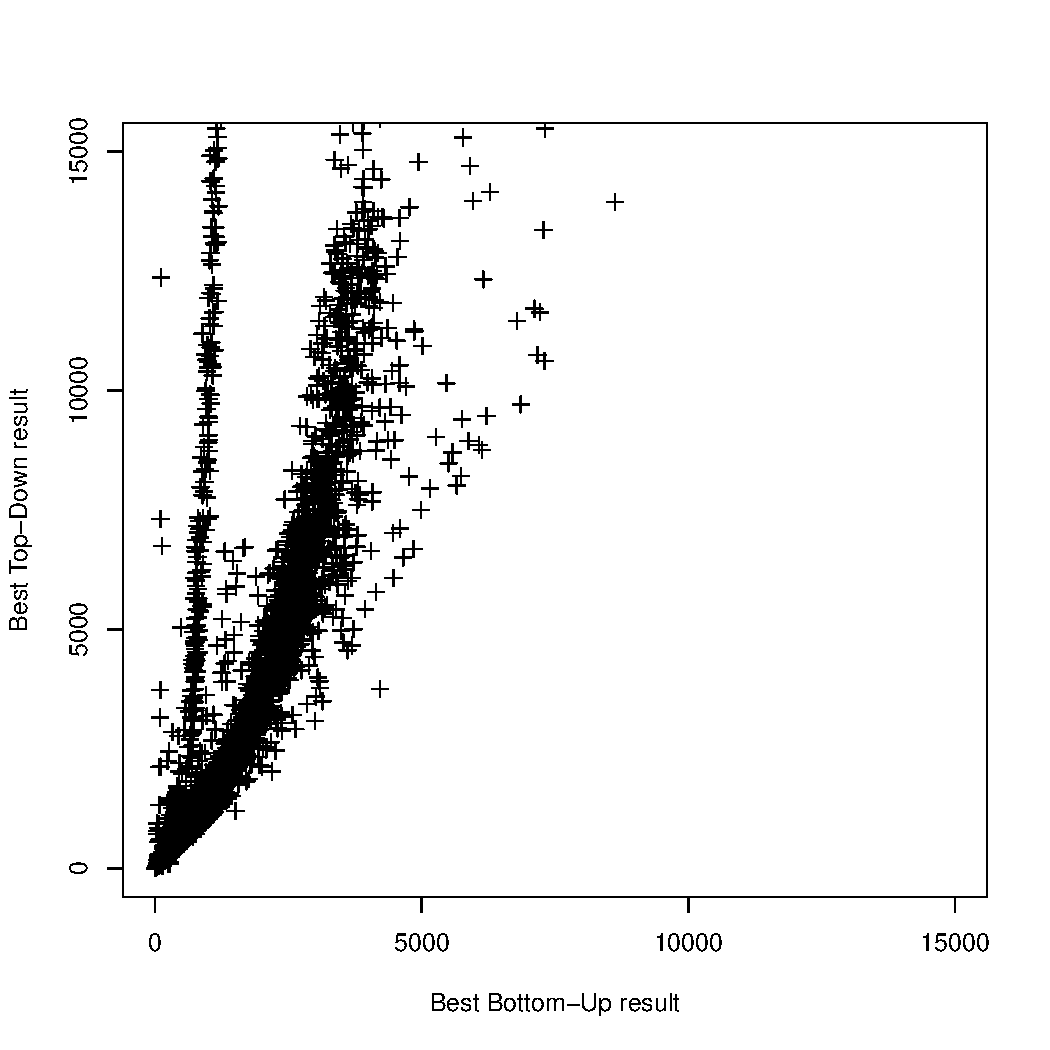
\includegraphics[scale=0.5]{chapters/pebbling/figures/td_vs_bu.pdf}
	\caption{Space measures of best Bottom-Up and Top-Down result}
	\label{fig:BUvsTD}
\end{figure}

The Bottom-Up algorithm does not only produce better results, it is also much faster, as can be seen in the last column of Table \ref{tab:results}. 
The reason probably is the number of comparisons that the algorithms make. 
For Bottom-Up the set $N$ of possible choices consists of the premises of a single node only, i.e. $|N| \in \{0,2\}$.
For Top-Down the set $N$ is the set of currently pebbleable nodes, which can be large (e.g. for a perfect binary tree with $2n -1$ nodes, initially $|N| = n$). 
Possibly for some heuristics, Top-Down algorithms could be made more efficient by using, instead of a set, an ordered sequence of pebbleable nodes together with their memorized heuristic evaluations.

Unsurprisingly the radius used for the Distance Heuristic has a severe impact on the speed, which decreases rapidly as the maximum radius increases. 
With radius 5, only a few small proofs were processed in a reasonable amount of time.

On average the smallest space measure of a proof is 44.1 times smaller than its length. 
This shows the impact that the usage of deletion information together with well constructed topological orders can have. 
When these techniques are used, on average 44.1 times less memory is required for storing nodes in memory during proof processing.


%%%%%%%%%%%%%%%%%%%%%%%%%%%%%%%%%%%%%%%%%
%%% Conclusion %%%%%%%%%%%%%%%%%%%%%%%%%%
%%%%%%%%%%%%%%%%%%%%%%%%%%%%%%%%%%%%%%%%%
%\chapter{Conclusion}
%\label{ch:conclusion}
%%%%%%%%%%%%%%%%%%%%%%%%%%%%%%%%%%%%%%%%%

%Several algorithms for compressing proofs with respect to space have been conceived. The experimental evaluation clearly shows that the so-called Bottom-Up algorithms are faster and compress more than the more natural, straightforward and simple Top-Down algorithms. Both kinds of algorithms are parameterized by a heuristic function for selecting nodes. The best performances are achieved with the simplest heuristics (i.e. Last Child and Number of Children). More sophisticated heuristics provided little extra compression but cost a high price in execution time. Future work could investigate heuristics that take advantage of the particular shape of proofs generated by analysis of conflict graphs.

\vspace{-5pt}
\paragraph{Acknowledgments:} We would like to thank Armin Biere for clarifying why resolution chains are not left-associative in the TraceCheck proof format.

\vspace{-5pt}





\bibliographystyle{splncs}
\bibliography{../jabref_references}


\end{document}

% vim: tw=100
